\documentclass[11pt,a4paper]{report}
\usepackage[utf8]{inputenc}
\usepackage[T1]{fontenc}
\usepackage{geometry}
\geometry{margin=1in}
\usepackage{graphicx}
\usepackage{setspace}
\usepackage{titlesec}
\usepackage{longtable}
\usepackage{array}
\usepackage{tikz}
\usepackage{hyperref}
\usepackage{enumitem}
\setcounter{secnumdepth}{3}
\renewcommand{\thesection}{\arabic{section}}
\setlength{\parskip}{4pt}
\begin{document}

% ------------------ Title Page ------------------
\begin{titlepage}
\centering
\IfFileExists{College Logo Grayscale.jpg}{
\includegraphics[width=3.4cm,height=2.6cm,keepaspectratio]{College Logo Grayscale.jpg}\\[0.5cm]}{\vspace*{2cm}}
\vspace{0.7cm}
\textbf{\large A Course End Project Report on}\\[0.5cm]
{\LARGE \textbf{Student Results and Grade Management System}}\\[1.2cm]
{\Large Software Development / Database Management Project}\\[1.3cm]
\textbf{Submitted by}\\[0.25cm]
Batch No.: {Enter Batch Number}
\begin{center}
\begin{tabular}{l l}
{Student Name 1} & {Roll Number 1}\\[2mm]
{Student Name 2} & {Roll Number 2}\\[2mm]
{Student Name 3} & {Roll Number 3}\\[2mm]
\end{tabular}
\end{center}
\textbf{Course Facilitator}\\[0.075in]
{Faculty Name}\\
{Designation}\\[2.2cm]
{\large\textbf{Department of {Department Name}}}\\[0.5cm]
{\large\textbf{{College Name, City}}}\\[0.5cm]
{\large \textbf{Academic Year 2025--2026}}
\end{titlepage}

\tableofcontents
\clearpage

\section*{Abstract}
\addcontentsline{toc}{section}{Abstract}
Managing student marks and preparing academic results manually can be slow, repetitive, and vulnerable to calculation and data-entry errors. The Student Results and Grade Management System is a software application designed to organize student details, subject-wise marks, totals, percentages, grades, and pass/fail status in a consistent way. The proposed educational prototype uses Java for application logic and MySQL for persistent data storage. Java Database Connectivity (JDBC) connects the application to the database, while parameterized \texttt{PreparedStatement} queries support safer insertion, retrieval, updating, and deletion of records.

The system calculates the total and average percentage from five subject marks and assigns a grade according to configurable demonstration rules. It allows an operator to insert a student result, view available results, search by roll number, update marks, and remove a record. Centralized storage can reduce duplicate record keeping and makes retrieval easier than paper-based methods or disconnected spreadsheets. The project demonstrates fundamental concepts in object-oriented programming, relational database design, SQL, validation, and software testing. It is a prototype rather than a production examination platform; real deployment would require institution-approved grading rules, secure authentication, role-based access, audit trails, backups, privacy controls, and extensive testing.

\textbf{Keywords:} Student information system, result management, grade calculation, Java, MySQL, JDBC, PreparedStatement, database application.

\section{Introduction}
Educational institutions maintain student profiles, course details, subject marks, examination results, and academic records. When these tasks are handled entirely through paper registers or separate spreadsheets, staff may need to repeat calculations and search multiple files. Common difficulties include arithmetic mistakes, duplicate records, inconsistent formats, delayed result preparation, and accidental loss or modification of data.

The Student Results and Grade Management System proposes a simple database-backed application for storing and processing student results. Each student is identified by a unique roll number. The operator enters the student's name, branch, academic year, and marks for five subjects. The application calculates the total, percentage, grade, and overall pass/fail status using predefined rules. Records can then be displayed, searched, updated, or deleted.

The project is intended for learning and demonstration. It shows how a Java application communicates with a relational database and how repeated operations can be organized into a menu-driven interface. The design can later be extended with a graphical user interface, student and faculty logins, downloadable mark sheets, multiple semesters, and web-based access.

\section{Literature Review}
Student information systems and learning-management platforms commonly combine student identity, course registration, assessment, and reporting functions. Spreadsheet applications are inexpensive and familiar, but they may rely on manual formulas and can become difficult to maintain when many users edit different copies. A relational database provides structured tables, unique identifiers, constraints, and query facilities that support consistent storage and retrieval.

Java is widely used for teaching object-oriented programming and database connectivity. JDBC provides a standard interface through which Java programs can connect to supported databases, execute SQL statements, and process query results. A \texttt{PreparedStatement} separates SQL structure from supplied values and helps reduce SQL-injection risk when used correctly. It also makes repeated parameterized operations easier to manage.

The proposed system focuses on a small, understandable set of features suitable for a course project. It is not intended to replace a complete institutional ERP or official examination system. Its main contribution is the integration of record management with automatic grade calculation in a compact prototype.

\section{Objectives}
\begin{itemize}
\item To store student details and subject-wise marks in a structured database.
\item To calculate total marks, percentage, grade, and pass/fail status automatically.
\item To provide options to insert, display, search, update, and delete student results.
\item To connect a Java application to MySQL using JDBC.
\item To use parameterized SQL queries for database operations involving user input.
\item To reduce repetitive manual calculations and improve the consistency of result records.
\item To demonstrate a design that can be expanded for multiple classes, semesters, and reports.
\end{itemize}

\section{Methodology}
The development process is divided into requirement analysis, system design, database creation, implementation, testing, and evaluation. First, the required student fields and operations are identified. Next, a relational table is designed with the roll number as the primary key. Java methods are then implemented for database connection, insertion, retrieval, updating, and deletion. Grade calculation is performed by application logic after validating the marks. Finally, sample records are used to test normal operations and boundary conditions.

\subsection{System Block Diagram}
\begin{figure}[ht]
\centering
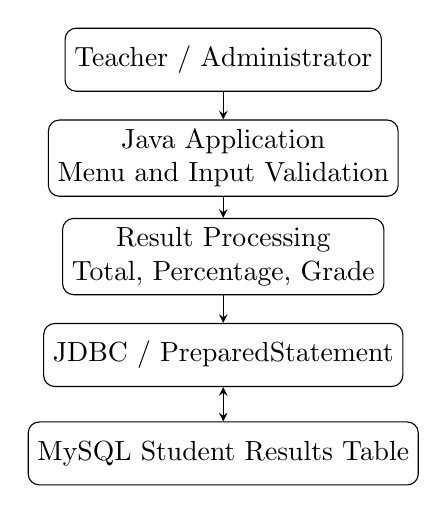
\begin{tikzpicture}[node distance=1.25cm, every node/.style={draw,rounded corners,align=center,minimum width=3.2cm,minimum height=0.8cm},>=stealth]
\node (user) {Teacher / Administrator};
\node (app) [below of=user] {Java Application\\Menu and Input Validation};
\node (logic) [below of=app] {Result Processing\\Total, Percentage, Grade};
\node (jdbc) [below of=logic] {JDBC / PreparedStatement};
\node (db) [below of=jdbc] {MySQL Student Results Table};
\draw[->] (user) -- (app);
\draw[->] (app) -- (logic);
\draw[->] (logic) -- (jdbc);
\draw[<->] (jdbc) -- (db);
\end{tikzpicture}
\caption{Block diagram of the Student Results and Grade Management System}
\label{fig:blockdiagram}
\end{figure}

\subsection{System Components}
\begin{itemize}
\item \textbf{User/operator:} Enters student details and chooses the required operation.
\item \textbf{Java application:} Displays the menu, accepts input, validates marks, and controls the workflow.
\item \textbf{Grade calculation module:} Calculates total marks and percentage, assigns a grade, and determines pass/fail status.
\item \textbf{JDBC:} Provides the connection between Java and MySQL.
\item \textbf{MySQL database:} Stores student information and calculated results persistently.
\item \textbf{PreparedStatement:} Executes parameterized SQL queries for insert, search, update, and delete operations.
\end{itemize}

\subsection{Database Design}
The database is named \texttt{college} and the main table is \texttt{student\_results}. The \texttt{roll\_no} field is the primary key, ensuring that two records cannot use the same roll number. The table stores student name, branch, academic year, five subject marks, total, percentage, grade, and result status. Numeric fields are stored using decimal types to retain fractional values where needed. Required fields are declared as \texttt{NOT NULL}.

\begin{longtable}{|p{3.4cm}|p{3.1cm}|p{7cm}|}
\caption{Main database fields}\\\hline
\textbf{Field} & \textbf{Type} & \textbf{Purpose}\\\hline
\endfirsthead
\hline \textbf{Field} & \textbf{Type} & \textbf{Purpose}\\\hline
\endhead
roll\_no & VARCHAR(20) & Unique student identifier and primary key.\\\hline
student\_name & VARCHAR(100) & Student's full name.\\\hline
branch & VARCHAR(30) & Academic department or branch.\\\hline
academic\_year & VARCHAR(20) & Year or class label.\\\hline
subject1--subject5 & DECIMAL(5,2) & Marks obtained in five subjects.\\\hline
total & DECIMAL(6,2) & Sum of the five subject marks.\\\hline
percentage & DECIMAL(5,2) & Average percentage across five equally weighted subjects.\\\hline
grade & VARCHAR(2) & Grade assigned from the percentage.\\\hline
result\_status & VARCHAR(10) & Overall PASS or FAIL status.\\\hline
\end{longtable}

\subsection{Working Principle}
\begin{enumerate}
\item The operator starts the Java program and the application connects to the MySQL database.
\item The application creates the results table if it does not already exist.
\item The operator chooses an operation from the menu.
\item For insertion, the operator enters the roll number, name, branch, academic year, and five marks.
\item The application checks that each mark is within the range 0 to 100.
\item The program adds the marks and calculates percentage as total divided by five.
\item The grade is assigned according to the configured grade ranges. The result is FAIL if any subject mark is below 35; otherwise, it is PASS.
\item A parameterized SQL query stores or updates the record. Display and search options retrieve records from the database.
\item The operator can repeat operations until choosing Exit.
\end{enumerate}

\subsection{Grade Calculation Rules}
The prototype uses five equally weighted subjects, each marked out of 100. Total marks are the sum of all subject marks, and percentage is calculated as the total divided by five. The sample grade mapping is shown below. These values are illustrative and must be replaced with the official rules of the relevant institution before real use.

\begin{center}
\begin{tabular}{|c|c|}\hline
\textbf{Percentage} & \textbf{Grade}\\\hline
90--100 & A+\\\hline
80--89.99 & A\\\hline
70--79.99 & B\\\hline
60--69.99 & C\\\hline
50--59.99 & D\\\hline
Below 50 & F\\\hline
\end{tabular}
\end{center}

\subsection{Software Implementation}
The application is written in Java and uses MySQL as its relational database. JDBC's \texttt{DriverManager} establishes the connection. The \texttt{PreparedStatement} class is used to pass user values separately from SQL commands. The \texttt{ResultSet} class reads query results. The project source code and SQL setup script are included with this report in the repository.

The main operations are:
\begin{itemize}
\item \textbf{Insert:} Saves student details, marks, total, percentage, grade, and result status.
\item \textbf{Display:} Lists the stored results in roll-number order.
\item \textbf{Search:} Finds a record using its roll number.
\item \textbf{Update:} Recalculates and updates marks and derived result fields.
\item \textbf{Delete:} Removes a student record after the roll number is supplied.
\end{itemize}

\section{Results and Discussion}
The prototype is designed to demonstrate the complete flow from data entry to persistent result storage. After a valid record is entered, the application calculates the total, percentage, grade, and pass/fail status and stores the values in MySQL. The display option retrieves stored records, while search provides access to an individual student's result. Update recalculates the derived values whenever marks change, helping keep them consistent with the entered marks.

The application uses a primary key to prevent duplicate roll numbers and prepared statements to parameterize user-supplied values. Input checks restrict marks to the range 0--100. Database connectivity still depends on a running MySQL server, a correctly configured Connector/J library, and valid credentials. The demonstration has not been independently performance-tested with a large institutional dataset; therefore, no claim of production-level speed or capacity is made.

\subsection{Testing Plan}
\begin{longtable}{|p{3cm}|p{5cm}|p{5.5cm}|}
\caption{Representative functional tests}\\\hline
\textbf{Test} & \textbf{Action} & \textbf{Expected outcome}\\\hline
\endfirsthead
\hline \textbf{Test} & \textbf{Action} & \textbf{Expected outcome}\\\hline
\endhead
Create table & Run table setup option or application startup & Results table exists and is ready for use.\\\hline
Insert valid record & Enter unique roll number and marks from 0 to 100 & Record is stored with calculated total, percentage, grade, and status.\\\hline
Duplicate roll number & Insert another record using an existing roll number & Database rejects the duplicate primary key.\\\hline
Display results & Select display option & Stored records are listed.\\\hline
Search existing student & Enter a known roll number & Matching student's summary is displayed.\\\hline
Search missing student & Enter an unknown roll number & A no-record-found message is displayed.\\\hline
Update marks & Change marks for an existing roll number & Marks and calculated result fields are updated.\\\hline
Delete record & Delete an existing roll number & The record is removed.\\\hline
Invalid mark & Enter a value below 0 or above 100 & Input is requested again.\\\hline
\end{longtable}

\subsection{Advantages}
\begin{itemize}
\item Reduces repeated manual arithmetic by calculating totals and grades automatically.
\item Stores records in a central database instead of separate paper files.
\item Supports searching and updating records using a unique roll number.
\item Demonstrates database connectivity and core CRUD operations in Java.
\item Can be expanded with a graphical interface, export features, and multiple semesters.
\end{itemize}

\subsection{Limitations and Future Scope}
The current version is a basic console-based educational prototype. It uses a single sample grading policy and five subjects. It does not include production authentication, different user roles, multi-semester support, attendance, result approval workflows, audit logs, or report-card PDF generation. Future versions can add a Swing or web interface, administrator and faculty accounts, password hashing, role-based permissions, subject configuration, CSV/PDF export, database backups, and a dashboard for performance analysis. Any real deployment should follow the institution's data-protection policies and approved grading rules.

\section{Mapping POs and SDGs}
\subsection{Program Outcomes (POs) Mapping}
\begin{center}
\small
\begin{tabular}{|c|p{5.1cm}|p{7cm}|}\hline
\textbf{PO} & \textbf{Program outcome} & \textbf{Project relevance}\\\hline
PO1 & Engineering knowledge & Applies programming, database, and software design concepts.\\\hline
PO2 & Problem analysis & Identifies errors and inefficiencies in manual result processing.\\\hline
PO3 & Design/development of solutions & Designs a structured system for managing marks and results.\\\hline
PO5 & Modern tool usage & Uses Java, JDBC, SQL, and MySQL tools.\\\hline
PO8 & Ethics & Highlights the need for confidentiality and responsible handling of student records.\\\hline
PO12 & Life-long learning & Provides a foundation for future study of web applications and database systems.\\\hline
\end{tabular}
\end{center}

\subsection{Sustainable Development Goals (SDGs) Mapping}
\begin{center}
\small
\begin{tabular}{|c|p{5cm}|p{7cm}|}\hline
\textbf{SDG} & \textbf{Goal} & \textbf{Project relevance}\\\hline
SDG 4 & Quality Education & Supports organized academic record management and access to results by authorized staff.\\\hline
SDG 9 & Industry, Innovation and Infrastructure & Demonstrates a practical digital information-management solution.\\\hline
SDG 12 & Responsible Consumption and Production & Can reduce reliance on repeated paper registers and printed working copies.\\\hline
\end{tabular}
\end{center}

\section{Conclusion}
The Student Results and Grade Management System demonstrates how Java and MySQL can be combined to manage student marks and academic results. The application supports inserting, displaying, searching, updating, and deleting records. It calculates totals, percentages, grades, and pass/fail status according to sample rules. The project provides practical experience with object-oriented programming, relational database design, JDBC, and parameterized SQL queries. Further work is needed to introduce secure authentication, institutional grading policies, multiple semesters, report generation, and production-level privacy and reliability controls.

\begin{thebibliography}{99}
\addcontentsline{toc}{section}{Bibliography}
\bibitem{java} Oracle, \textit{Java Documentation}. Available: \url{https://docs.oracle.com/en/java/}
\bibitem{jdbc} Oracle, \textit{JDBC Basics}. Available: \url{https://docs.oracle.com/javase/tutorial/jdbc/basics/}
\bibitem{mysql} Oracle, \textit{MySQL Reference Manual}. Available: \url{https://dev.mysql.com/doc/}
\bibitem{owasp} OWASP Foundation, \textit{SQL Injection Prevention Cheat Sheet}. Available: \url{https://cheatsheetseries.owasp.org/cheatsheets/SQL_Injection_Prevention_Cheat_Sheet.html}
\bibitem{silberschatz} A. Silberschatz, H. F. Korth, and S. Sudarshan, \textit{Database System Concepts}. McGraw-Hill.
\end{thebibliography}
\end{document}
